\documentclass[10pt,a4paper]{article}
\usepackage[utf8]{inputenc}
\usepackage[francais]{babel}
\usepackage[T1]{fontenc}
\usepackage{amsmath}
\usepackage{amsfonts}
\usepackage{amssymb}
\usepackage{graphicx}
\author{Raphaël Mathon}
\title{Vol stationnaire autonome d'un quadrirotor}

\begin{document}

\maketitle

\part{Conception}

\section{Modélisation cinématique}

\subsection{Paramétrage}
Afin de simplifier l'étude dynamique et centrer notre étude sur la démarche d'asservissement du système, on décide de considérer le mouvement du drone suivant un unique degré de liberté, l'angle de roulis. Cela revient à considérer que le système est en liaison pivot avec le "bâti", qui est ici le référentiel terrestre.

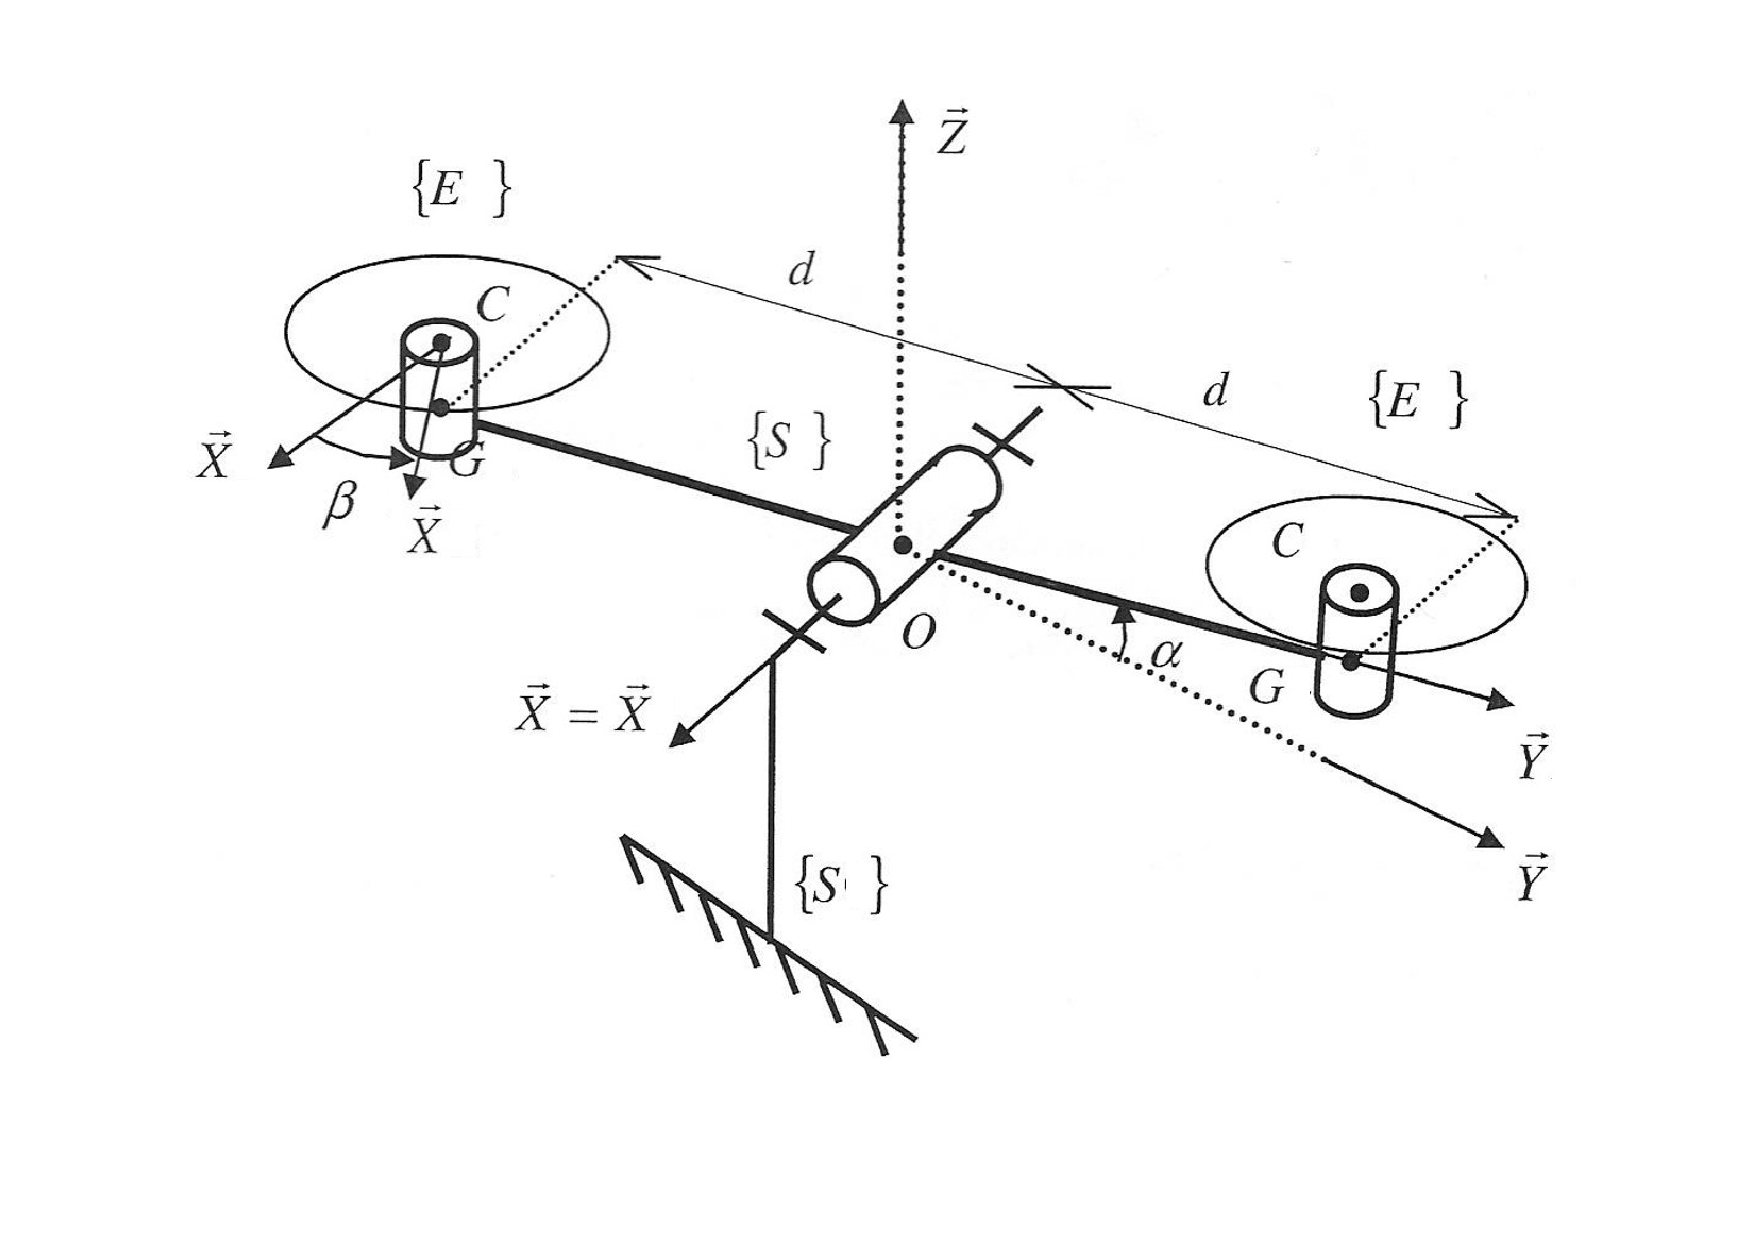
\includegraphics[scale=0.4]{schemaCinematique.pdf}

\section{Aérodynamique des hélices}

On souhaite dans cette section réaliser une modélisation de l'action de l'air sur les hélices du quadricoptère. En effet, afin de se maintenir en vol stationnaire, la rotation des hélices assure une portance suffisante pour compenser le poids. 

\subsection{Torseur d'action mécanique}

Les actions aérodynamiques s'expriment :

\begin{eqnarray}
\vec{Ft_{i}} = \frac{1}{2} \rho C_{t} S v^2 \vec{x_{i}} \\
\vec{Fp_{i}} = \frac{1}{2} \rho C_{p} S v^2 \vec{x_{i}}
\end{eqnarray}

Où:

\begin{itemize}
\item $\rho = 1.225$ $kg$ $m^{-3}$ : masse volumique de l'air
\item $C_{t}$, $C_{p}$ : coefficients de trainée et de portance
\item $S$ : surface caractéristique du solide
\item $v$ : vitesse apparente de l'air dans le référentiel du solide
\end{itemize} 

On considère le drone en vol stationnaire dans le référentiel terrestre supposé galiléen, noté $R_{0}$. On adopte la paramétrisation suivante: 

\begin{itemize}
\item Châssis+stator: $(E_{1})$ fixe dans $R_{0}$ : base $B_{1} = 
( \vec{x_{1}} , \vec{y_{1}} , \vec{z_{1}} )$,
\item rotor+hélice: $(E_{i})$ : base $ B_{i} = 
( \vec{x_{i}} , \vec{y_{i}} , \vec{x_{i}})$
\end{itemize}

$(E_{i})$ est en liaison pivot d'axe $(C,\vec{z_{1}})$ par rapport à $E_{i}$ autour de $ \vec{z_{1}} = \vec{z_{i}}$;
on pose $ \beta_{i} = (\vec{x_{1}},\vec{x_{i}}) = (\vec{y_{1}},\vec{y_{i}}),
\dot \beta_{i} = \dfrac{d\beta_{i}}{dt}$

Considérons un élément de pale infinitésimal de longueur $dr$ et d'épaisseur $e$ situé en $M$, où $ \vec{CM}=r \vec{u_{x_{2}}} $.
La vitesse de rotation de l'hélice est très élevé, ainsi :
 \\
$$ \vec{v}(M,air/E_{i}) = -\vec{v}(M,2/1) = -r \dot \beta_{i} \vec{y_{i}}$$

On exprime alors le torseur global de l'action de l'air sur l'hélice, considérée bipale et symétrique:

\begin{equation}
\lbrace \mathcal{T}(air \rightarrow E_{i}) \rbrace = 
\left\{ \begin{array}{c} \vec{\mathcal{R}_{i}} = 
2\int \limits_{0}^{R} { \frac{1}{2} \rho C_{p} S r^2 \dot \beta_{i}^2 \ e dr \ \vec{z_{1}} } \\
\vec{\mathcal{M}_{i}}(O) = 
-2\int \limits_{0}^{R} { \frac{1}{2} \rho C_{t} S r^3 \dot \beta_{i}^2 \ e dr } \ \vec{z_{1}}

\end{array} \right\}_{(C)}
\end{equation}

Puis, en intégrant et en exprimant en fonction du diamètre de l'hélice $D$ :

\begin{equation}
\lbrace \mathcal{T}(air \rightarrow E_{i}) \rbrace = 
\left\{ \begin{array}{c} \vec{\mathcal{R}_{i}} = 
\frac{1}{24} \rho e C_{p} D^3 \dot \beta_{i}^2 \ \vec{z_{1}}
 \\
\vec{\mathcal{M}_{i}}(O) = 
- \frac{1}{64} \rho e C_{t} D^4 \dot \beta_{i}^2 \ \vec{z_{1}}

\end{array} \right\}_{(C)}
\end{equation}

On retiendra finalement l'expression de la résultante, nécessaire dans le bilan des actions mécaniques extérieures du système $E$ :

\begin{equation}
\vec{\mathcal{R}_{i}} = K_{h} \dot \beta_{i}^2 \ \vec{z_{1}}
\end{equation}

Où :

\begin{equation}
K_{h} = \frac{1}{24} \rho e C_{p} D^3
\end{equation}

\subsection{Puissance}

La connaissance de ce torseur d'action permet le calcul de la puissance fournie par l'hélice à l'air :

\begin{equation}
\mathcal{P}_{i}(air \rightarrow E_{i}, R_{0}) =
\lbrace \mathcal{T}(air \rightarrow E_{i}) \rbrace _{(C)} \otimes
\lbrace \mathcal{V}(E_{i} / R_{0} \rbrace _{(C)}
\end{equation}

Ainsi : 

\begin{equation}
\mathcal{P}_{i}(air \rightarrow E_{i}, R_{0}) =
- \frac{1}{64} \rho e C_{t} D^4 \dot \beta_{i}^3 
\end{equation}

Cette puissance est négative : en effet, ce sont les actionneurs du drone qui fournissent une certaine puissance afin de mettre en mouvement l'air.

Afin d'évaluer numériquement les composantes du torseur d'action ou la puissance consommée, il est nécessaire de déterminer la valeur des coefficients aérodynamiques. Parmi les solutions envisageables, on en retient deux que l'on pourra comparer.

La première méthode consiste à modéliser chaque élément de pale par une section de profil standard dont les coefficients sont inscrits dans des bases de données, comme la base NACA. A partir de la mesure de grandeurs caractéristiques sur une photo du profil d'une hélice, on pourra trouver le profil adapté et lire la valeur de $C_{t}$ et $C_{p}$.

Une deuxième méthode est de déterminer ces coefficients à partir de mesures expérimentales fournies par les constructeurs de composants de drone. Notamment, en connaissant la poussée exercée par l'hélice et la puissance consommée pour plusieurs valeurs de $\beta_{i}$, il est possible de calculer ces coefficients.

Comme les valeurs de $C_{t}$ et $C_{p}$ ne dépendent que de la forme de l'hélice, on pourra conserver leurs ordres de grandeur pour des hélices de diamètres différents.

\section{Modélisation des moteurs}

\subsection{Spécificité des moteurs à courant continu sans balais}

Les moteurs à courant continu sans balais sont très répandus dans le milieu de l'aéromodélisme, et dans les applications de faible puissance en général (robotique, informatique...). Ces moteurs sont alimentés en courant continu; un composant électronique, l'ESC (electronic speed controller : variateur de vitesse électronique) assure la commutation des courants au sein du circuit statorique triphasé. 

Les moteurs brushless s'affranchissent des contraintes des balais et collecteurs équipant les MCC (frottements, remplacement, bruit), le rotor étant constitué d'aimants permanents. Cependant, afin d'assurer l'orthogonalité du champ magnétique statorique et du moment magnétique rotorique, le variateur de vitesse doit disposer de capteurs retournant la position du champ magnétique : pour les variateurs de vitesse de drones, il s'agit généralement de capteurs de force contre-electromotrice (technologie non détaillée ici).

\subsection{Equations}

La modélisation d'un moteur brushless est identique à celle d'un MCC (cf cours de génie mécanique, ENS Cachan). On retrouve les équations, dans l'hypothèse d'inductance faible des phases ($\frac{L}{R} <<1$) :

\begin{eqnarray}
C_{M_{i}} = K_{c} I_{i} \\
E_{i} = K_{c} \beta_{i} \\
I_{i} = \frac{U_{i} - E_{i}}{R} \\
J \dot \beta_{i} = C_{M_{i}} - C_{R_{i}}
\end{eqnarray}

Où : 

\begin{itemize}
\item $C_{M_{i}}$ : couple moteur
\item $C_{R_{i}}$ : couple résistant
\item $\beta_{i}$ : vitesse de rotation du rotor
\item $J$ : inertie du moteur
\item $K_{C}$ : constante de flux
\item $U_{i}$ : tension d'induit
\item $E_{i}$ : force contre-électromotrice
\item $I_{i}$ : courant d'induit
\end{itemize} 

On fait ainsi l'hypothèse que les deux moteurs ont des caractéristiques identiques.

On peut dès lors modéliser un tel moteur par un schéma bloc constitué des différentes équations dans le domaine de Laplace.

La section précédente a permis de modéliser le couple résistant $C_{R_{i}}$ exercé par l'air sur le rotor $E_{i}$. On verra par la suite s'il est important d'en tenir compte dans la modélisation globale de notre système.

Sans tenir compte du couple résistant, la fonction de transfert du moteur est alors :
\begin{equation}
H_{m_{i}}(p) = \frac{K_{m}}{1 + \tau p}
\end{equation}

Où $K_{m}$ et $\tau$ s'expriment en fonction des caractéristiques du moteur :

\begin{eqnarray}
K_{m} = \frac{1}{K_{c}} \\
\tau = \frac{R J}{K_{c}^2}
\end{eqnarray}



\section{Eléments dynamiques du système}

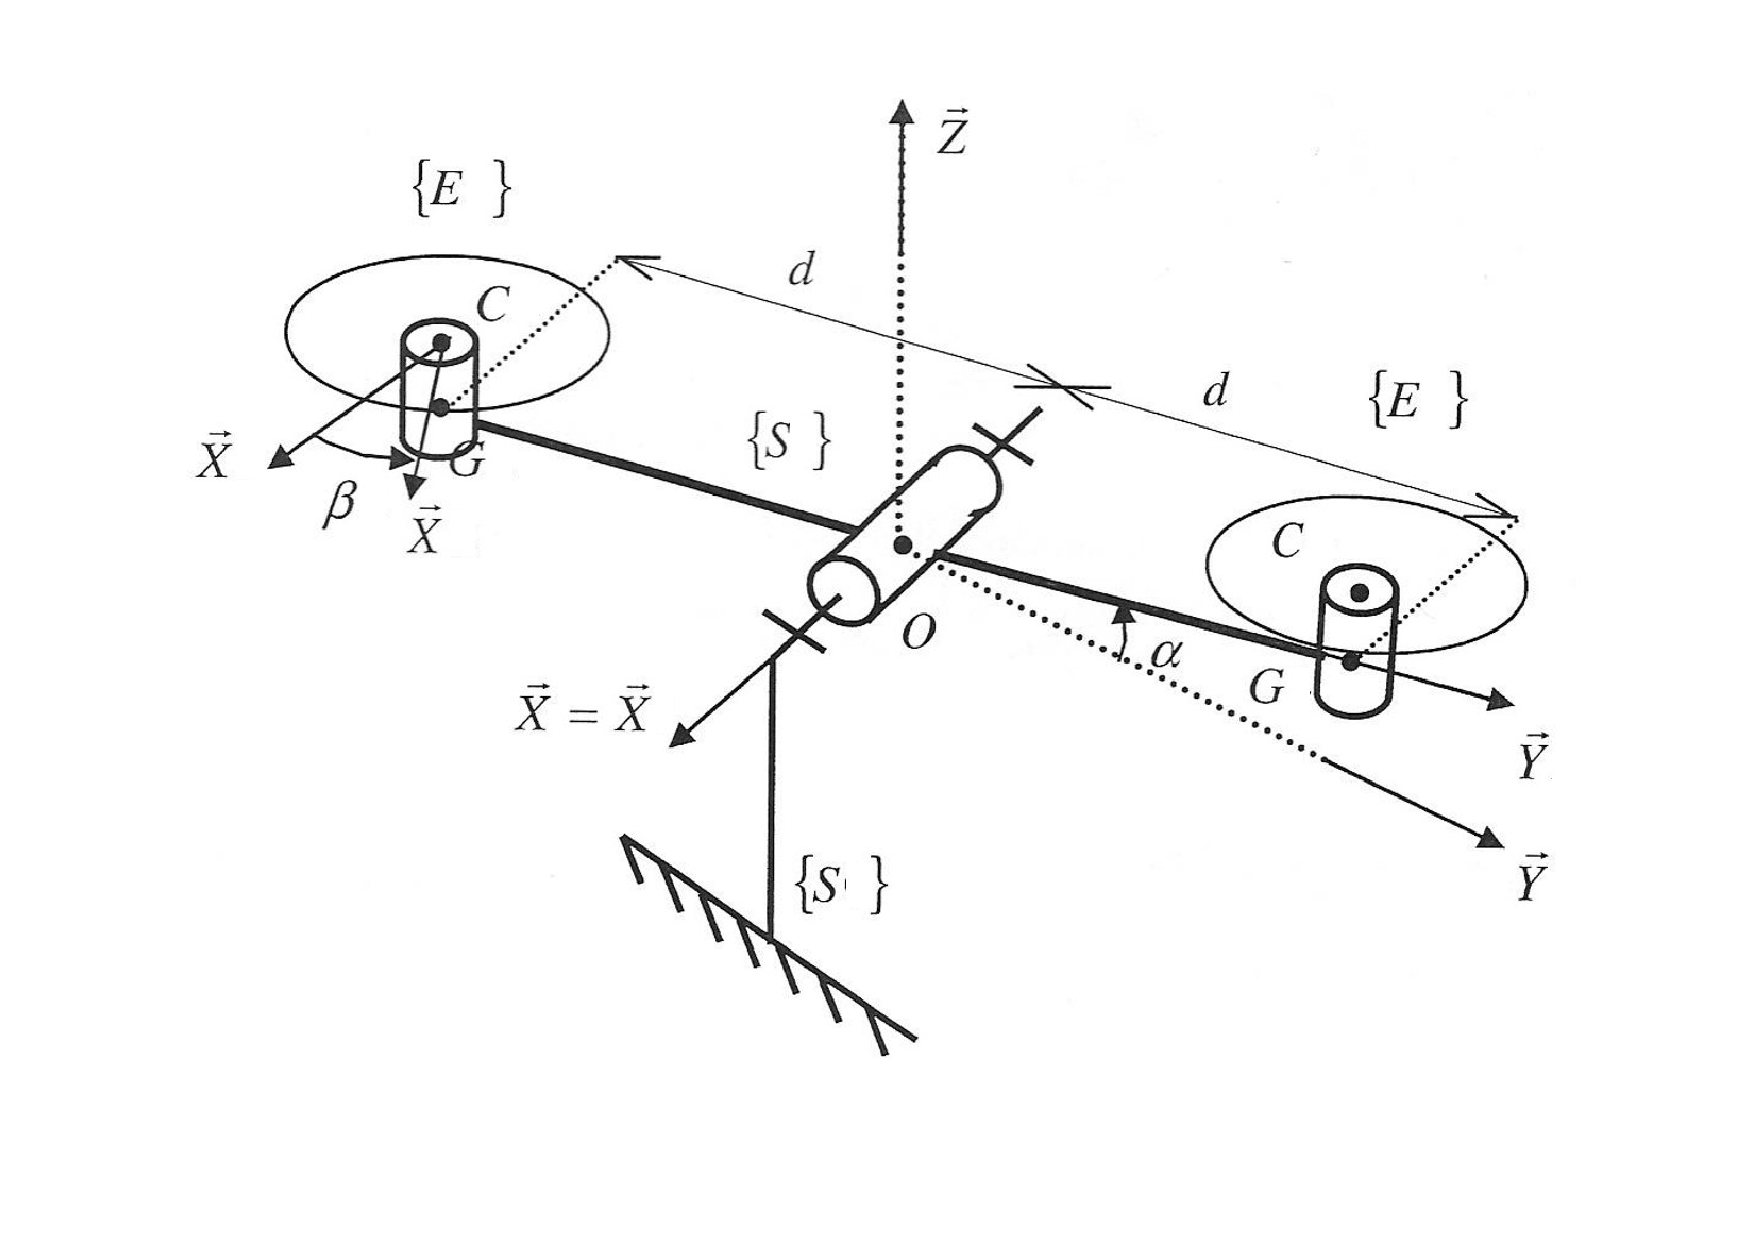
\includegraphics[scale=0.2]{schemaCinematique.pdf}

Considérons le système (E) constitué de deux hélices $E_{2}$ et $E_{3}$ en rotation autour des axes respectifs $(C_{2},\vec{z_{2}})$ et $(C_{3},\vec{z_{3}})$

\subsection{Hypothèses}
On fait les hypothèses suivantes : 
\begin{itemize}
\item Les solides $E_{i}$, constitués du rotor du moteur et de l'hélice, sont modélisés par des solides de révolution autour de leur axe de rotation. Le centre de l'hélice est noté $C_{i}$, le centre d'inertie est noté $G_{i}$.
\item L'ensemble $(E)$ est supposé parfaitement équilibré en terme de répartition de masse.
\item La liaison pivot est supposée parfaite.
\end{itemize}

\subsection{Eléments dynamiques}
En considérant l'hélice comme un solide de révolution autour de son axe de rotation, on peut considérer que sa matrice reste diagonale dans le repère $R_{1}$ et ainsi : \\
$
I(G_{2},E_{2}) = 
\begin{bmatrix}
I_{xx} & 0 & 0 \\
0 & I_{yy} & 0 \\
0 & 0 & I_{zz}
\end{bmatrix} _{R_{2},R_{1}}
$
, 
$
\vec{\Omega}(E_{2}/R_{0}) = 
\begin{bmatrix}
\alpha \\
0 \\
\beta_{2}
\end{bmatrix} _{R_{1}}
$ \\

Dans ce cas : \\
$
\vec{\sigma}(G_{2},E_{2}/R_{0}) = 
\left[ I(G_{2},E_{2}) \right] _{R_{1}}
\left[ \vec{\beta_{2}}(G_{2},E_{2}/R_{0}) \right] _{R_{1}}
 = 
 I_{xx} \dot \alpha \ \vec{x}_{1} + I_{zz} \dot \beta_{2} \ \vec{z}_{1}
$ \\

Puis en dérivant par rapport à $t$ en $R_{0}$ : \\
$
\vec{\delta}(G_{2},E_{2}/R_{0}) = 
I_{xx} \ddot \alpha \ \vec{x}_{1}
- I_{zz} \dot \beta_{2} \dot \alpha \ \vec{y}_{1}
+ I_{zz} \ddot \beta_{2} \ \vec{z}_{1}
$ \\

Soit : \\
$
\vec{\delta}(G_{2},E_{2}/R_{0}) =
\begin{bmatrix}
I_{xx} \ddot \alpha \\
- I_{zz} \dot \beta_{2} \dot \alpha \\
I_{zz} \ddot \beta_{2}
\end{bmatrix} _{R_{1}}
$ \\

On obtient finalement en changeant de point le moment dynamique de l'hélice au point $O$ : \\
$
\vec{\delta}(O,E_{2}/R_{0}) =
\begin{bmatrix}
(I_{xx} + m d^2) \ddot \alpha \\
- I_{zz} \dot \beta_{2} \dot \alpha \\
I_{zz} \ddot \beta_{2}
\end{bmatrix} _{R_{1}}
$ \\

Le calcul étant identique pour l'hélice $E_{3}$ : \\
$
\vec{\delta}(O,E_{3}/R_{0}) =
\begin{bmatrix}
(I_{xx} + m d^2) \ddot \alpha \\
- I_{zz} \dot \beta_{3} \dot \alpha \\
I_{zz} \ddot \beta_{3}
\end{bmatrix} _{R_{1}}
$ \\

D'autre part, on obtient de même la moment dynamique du châssis $E_{1}$ en $O$ : \\
$
\vec{\delta}(O,E_{1}/R_{0}) =
\begin{bmatrix}
I_{0xx} \ddot \alpha \\
0 \\
0
\end{bmatrix} _{R_{1}}
, \ 
I(O,E_{1}) = 
\begin{bmatrix}
I_{0xx} & 0 & 0 \\
0 & I_{0yy} & 0 \\
0 & 0 & I_{0zz}
\end{bmatrix} _{R_{1}}
$ \\

Finalement :

\begin{equation}
\vec{\delta}(O,E/R_{0}) =
\begin{bmatrix}
( 2 (I_{xx} + m d^2) + I_{0xx}) \ddot \alpha \\
- I_{zz} \dot \alpha ( \dot \beta_{2} + \dot \beta_{3} ) \\
I_{zz} ( \ddot \beta_{2} + \ddot \beta_{3} )
\end{bmatrix} _{R_{1}}
\end{equation}

\subsection{Théorème du moment dynamique}
On peut finalement appliquer le théorème du moment dynamique au système $E$ en $O$ selon l'axe $(O,\vec{x}_{1})$. Les moments de l'action de l'air sur les hélices sont : \\
$
\vec{\mathcal{M}}(O,air \rightarrow E2) = - d K_{h} \dot \beta_{2}^2 \  \vec{x}_{1}
\ , \  
\vec{\mathcal{M}}(O,air \rightarrow E3) = + d K_{h} \dot \beta_{3}^2 \  \vec{x}_{1}
$ \\
Soit finalement : 

\begin{eqnarray}
J_{eq_{x}} \ddot \alpha = d K_{h} (\dot \beta_{3}^2 - \dot \beta_{2}^2 ) \\
Jeq_{x}= 2 (I_{xx} + m d^2) + I_{0xx}
\end{eqnarray}



Où :
\begin{itemize}
\item $K_{h}$ : coefficient de portance de l'hélice (défini précédemment)
\item $Jeq_{x}$ : inertie équivalente de $E$ par rapport à l'axe $(O,\vec{x_{1}})$
\end{itemize}

\end{document}